% !TeX encoding = UTF-8
% !TeX program = pdflatex
% !TeX spellcheck = it_IT
\documentclass[binding=0.6cm]{sapthesis}
\usepackage[hidelinks]{hyperref}
\usepackage[italian]{babel}
\usepackage[utf8]{inputenc}
\usepackage{tcolorbox}
\usepackage{microtype}
\usepackage{longtable}
\usepackage{fancyvrb}
\usepackage{amsfonts}
\usepackage{animate}
\usepackage{float}

\newtcolorbox{codebox}{colback=darkgray!10!white, colframe=black}

\hypersetup{pdftitle={Simulazione di trading agents}, pdfauthor={Sebastiano Deodati}}

\title{Simulazione di trading agents}
\author{Sebastiano Deodati}
\IDnumber{2025953}
\course{Laurea Triennale in Informatica}
\courseorganizer{Facoltà di Ingegneria dell'informazione, Informatica e Statistica}
\AcademicYear{2024/2025}
\advisor{Prof. Enrico Tronci}
\authoremail{deodati.2025953@studenti.uniroma1.it}
\copyyear{2025}
\thesistype{Tesi di Laurea Triennale}

\begin{document}
	\frontmatter
	\maketitle
	\begin{abstract}
		L'oggetto di questa tesi è la progettazione di \textbf{trading agents} e la loro validazione tramite simulazioni di trading su dati storici. I trading agents sono sistemi che si occupano di fare
		trading online, e in queste pagine analizzeremo le sfide che si presentano nel design di questi sistemi, che hanno l'arduo compito di \textit{dare un senso} al caos che è il mercato azionario. \\
		In particolare, studieremo come diverse tecniche di \textbf{\textit{machine learning}}, semplici ma potenti, possano venire in nostro aiuto e fare una grande differenza. \\
		La tesi è suddivisa fondamentalmente in quattro parti: nei primi due capitoli analizzeremo il problema ed introdurremo le tecniche di machine learning utilizzate, nei tre capitoli successivi entreremo
		nel vivo del design di sistemi software in grado di sfruttare il machine learning per ottimizzare il trading online, il capitolo 6 è dedicato alla progettazione di trading agents capaci di gestire più
		titoli contemporaneamente, e nei due capitoli finali ci dedicheremo alla simulazione degli agents e analizzeremo i risultati formulando giudizi sui diversi approcci esplorati.
	\end{abstract}
	\tableofcontents
	\mainmatter
	\chapter{Introduzione ai trading agent}
		\section{Introduzione al trading online}
			Il \textbf{trading online} è la compravendita di strumenti finanziari (come azioni, obbligazioni, futures, titoli di Stato, criptovalute ecc.) tramite Internet. I principali vantaggi degli
			strumenti di questo tipo sono i minori costi di commissione richiesti all'investitore e soprattutto la possibilità, tramite appositi software detti \textbf{trading agent}, di automatizzare
			le operazioni di compravendita a fronte di un minore rischio associato all'errore umano grazie ad un'analisi automatizzata delle condizioni del mercato e quindi ad una più efficace
			rilevazione delle finestre di opportunità di acquisto e di vendita.
		\section{Definizione di trading agent}
			Un \textbf{trading agent} è un agente il cui compito è di osservare il mercato azionario e compravendere titoli in modo automatico al fine di avere un guadagno. Negli ultimi anni hanno
			acquisito sempre più rilevanza, basti pensare al fatto che nel 2014 oltre il 75 per cento delle negoziazioni sui mercati degli Stati Uniti (tra cui il New York Stock Exchange e Nasdaq)
			provenivano da sistemi di trading automatico. La maggiore sfida consiste nell'impostare la giusta strategia di individuazione di trend, dove gli approcci sono i più disparati. In particolare
			noi tratteremo di come diverse tecnologie di \textit{machine learning}, supportate da strumenti matematici e statistici convenzionali, possano dimostrarsi decisamente efficaci per tale scopo.
		\section{Definizione di machine learning}
			Il \textbf{machine learning} (ML) è un ambito dell'intelligenza artificiale il cui obiettivo è studiare modelli in grado di prendere decisioni autonomamente regolando i propri parametri interni
			in funzione di dati osservati. Vista la crescita esponenziale di questo approccio, dovuto alla sua elevata flessibilità, oggi è alla base della maggior parte dei modelli di intelligenza
			artificiale, diventando i due termini (\textit{erroneamente}) quasi sinonimi. Le tecniche di machine learning qui trattate sono abbastanza semplici e non sono che una goccia nell'oceano di
			modelli ben più potenti (basti pensare ai principali \textit{LLM} o a modelli di forecasting come \underline{\href{https://facebook.github.io/prophet/}{Facebook Prophet}}).
		\section{Machine learning per l'individuazione di trend nei prezzi}
			Individuare trend nei prezzi al fine di trovare i momenti ottimali per comprare è una grande sfida, vista la caoticità e la volatilità del mercato, e richiede una certa velocità nel prendere
			decisioni e nel comprare/vendere, motivo per cui fare trading in maniera manuale non è fattibile, e ciò rende necessario sviluppare un trading agent che operi in maniera del tutto autonoma e
			che sappia riconoscere le finestre di opportunità per comprare e vendere. Per fare ciò si può ricorrere a strumenti statistici convenzionali (valutare medie a breve e lungo termine, valutare la
			varianza dei prezzi ecc.) anche con un certo successo, tuttavia le opportunità offerte dal machine learning da questo punto di vista sono immense, con la possibilità di addestrare modelli a
			individuare tutti i possibili indicatori statistici nascosti che una logica deterministica, o meglio ancora l'occhio umano, non sarebbero mai in grado di cogliere.
	\chapter{Tecniche di machine learning}
		\section{Reti neurali}
			\subsection{Definizione}
				Una \textbf{rete neurale} è un modello computazionale ampiamente utilizzato in machine learning, dove si ha una rete di "neuroni" artificiali interconnessi che, imitando vagamente il
				modello biologico a cui si ispirano, si scambiano segnali che vengono processati da ogni singolo nodo ("neurone") che attraversano. Questi modelli sono in grado di individuare relazioni
				sia di tipo lineare che nonlineare tra dei segnali di input e dei segnali di output attesi, tramite un processo di aggiustamento dei parametri della rete detto \textit{training}. Per questa
				loro proprietà le reti neurali sono classificate come approssimatori universali di funzioni, e per questo sono molto indicate per accellerare processi computazionali molto complessi o, nel
				nostro caso, "automatizzare" l'analisi di trend statistici al fine di approssimare una funzione nonlineare.
			\subsection{Training problem}
				Il \textbf{training} di una rete neurale consiste nel trovare una soluzione al \textbf{training problem}, cioè risolvere il problema di ottimizzazione quadratico:
				\[
					\min_{A,b,r}
					\sum_{s=1}^q
					\mathcal{L} \Biggl(
						\sum_{\ell=1}^m
						r_\ell \,\sigma\bigl((A\,y(x^s) + b)_\ell\bigr)
						,\;\beta^s
						\Biggr)
				\]
				Dove le coppie $(x^s, \beta^s)$ sono le coppie (input, valore atteso) provenienti dal dataset e $\mathcal{L}$ è la funzione di loss, cioè una funzione che misura il
				grado di errore di una predizione, ovvero la distanza tra valore atteso e predizione della rete. \\
				Questo aspetto è gestito in maniera automatica da tutti i principali framework di machine learning, i quali mettono a disposizione funzioni di libreria per tale scopo, che tendenzialmente si
				appoggiano a discesa del gradiente.
				Per il training delle reti usate di seguito è stata scelta come funzione di \textit{loss} (funzione obiettivo da minimizzare) \textit{Huber loss}, così definita
				\[
					\mathcal{L}_{\delta }(a)={
						\begin{cases}
						{
							\frac{1}{2}}{a^{2}} &{ \text{per }|a|\leq \delta }, \\
							\delta \cdot \left(|a|-{\frac {1}{2}}\delta \right) &{ \text{altrim.}
						}
						\end{cases}
					}
				\]
				e come ottimizzatore è stato scelto \textit{AdamW}.
				\label{fig:nn}
				\begin{figure}[H]
				{
					\centering
					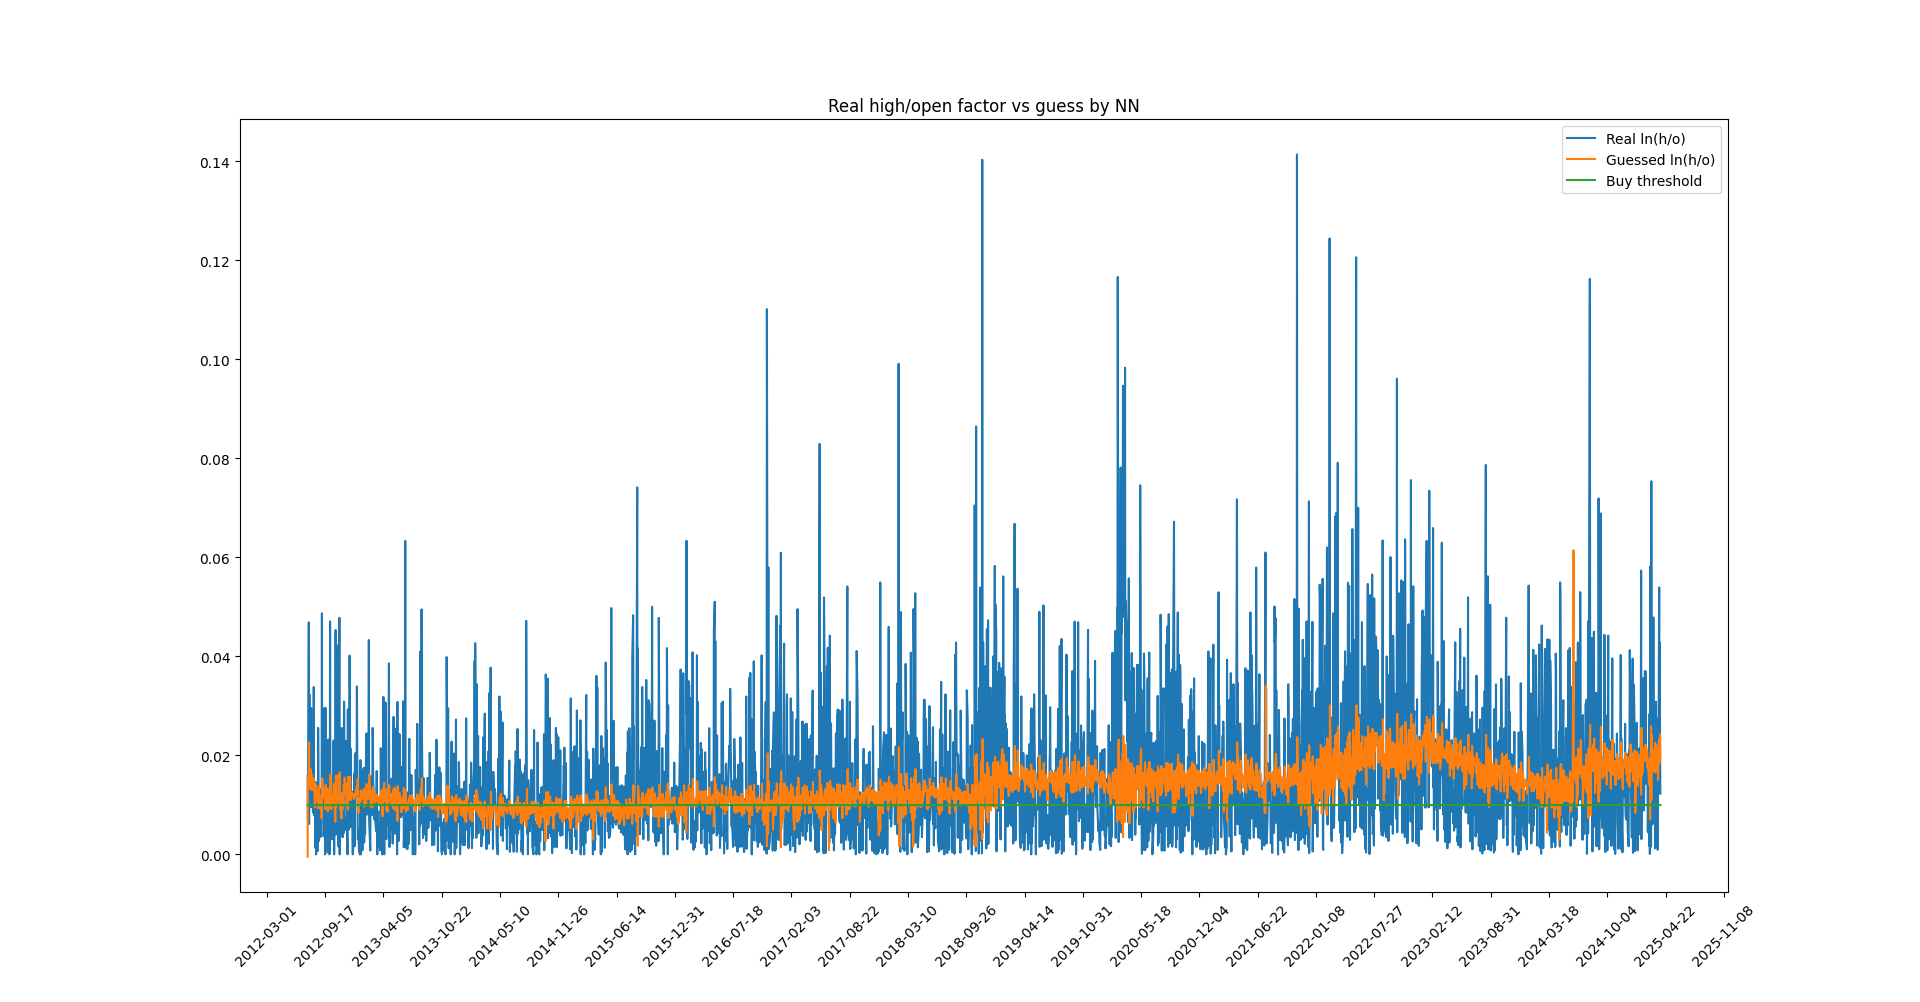
\includegraphics[width=0.8\linewidth]{assets/nn_plot_nvda.png}
					\caption{Time series del rapporto high/open di NVDA reale vs la time series approssimata dal modello}
				}
				\end{figure}
				Dalla figura si nota come, malgrado l'approssimazione non sia esatta, la rete riesce comunque a catturare il trend del prezzo, avendo una versione "meno rumorosa" della time 
				series reale.
		\section{Regressione lineare}
			\subsection{Definizione}
				La regressione lineare è essenzialmente una tipologia di machine learning molto basilare, è un modello statistico atto a stimare la relazione tra un insieme di variabili indipendenti (regressori)
				e una variabile dipendente da esse. Un modello di regressione lineare calcola la best fit, cioè la retta che meglio approssima la relazione tra tali fattori, che ha quindi equazione:
				\[ \hat{y} = \theta_0 + \theta_1x_1 + \theta_2x_2 + ... + \theta_nx_n \]
				dove $\hat{y}$ è l'approssimazione della variabile dipendente e $x_1 x_2 \,...\, x_n$ le variabili indipendenti e $\theta_1 \theta_2 ... \theta_n$ i coefficienti, e $\theta_0$ l'intercept
				(soluzione per $[x_0 \,...\, x_n] = [0 \,...\, 0]$). Abbiamo quindi che lo slope (inclinazione della retta) è uguale a $\theta_1x_1 + \theta_2x_2 + ... + \theta_nx_n$. \\
				Per i nostri scopi, la variabile indipendente è una sola ed è il tempo, mentre la variabile dipendente è il prezzo (in particolare, ci interessa il prezzo di \textit{close}), vogliamo cioè
				"prevedere il futuro" stimando il valore di $Y$ in istanti $X$ futuri. Per fare ciò, all'inizio della giornata di trading, l'agent troverà la best fit sulla sliding window di dimensione $W$
				$close_t-W...close_{t-1}$, avendo quindi una previsione di $close_t$ da utilizzare nella decisione di \textit{buy}. \\
				Basandosi su queste ipotesi si utilizza un algoritmo di discesa del gradiente per minimizzare l'errore quadratico medio (\textit{Mean Squared Error}, \textit{MSE}), che misura la distanza tra
				i valori reali osservati e l'approssimazione lineare, ed è definita come
				\[ MSE = \frac{1}{n} \sum_{i=1}^{n} (y_i - \hat{y}_i)^2 \]
				dove $y_i$ è il valore reale osservato nel punto $x_i$, mentre $\hat{y}_i$ è il valore attuale della regressione lineare nel punto $x_i$.
			\subsection{Regressione lineare semplice}
				\begin{figure}[H]
				{
					\centering
					\animategraphics[
						loop, autoplay, width=0.8\linewidth
					]{30}{assets/lr/lr-}{1}{874}
					\caption{Dimostrazione di come la regressione lineare può catturare trend in una time series}
				}
				\end{figure}
				Quando una regressione lineare ha un solo regressore è detta regressione lineare semplice. Dal momento che il nostro scopo è prevedere andamenti nei prezzi in funzione del tempo, ovvero la nostra
				variabile indipendente è il tempo, questo è il nostro caso, e la regressione lineare avrà quindi forma:
				\[ \hat{y}(t) = \theta_0 + \theta_1t \]
				dove $\hat{y}(t)$ è l'approssimazione della variabile dipendente (per noi il prezzo) nell'istante di tempo $t$.
				Per le nostre applicazioni andremo quindi a risolvere il problema di ottimizzazione:
				\[
					\min_{\theta_0,\theta_1}
					\sum_{s=1}^k
					\Biggl(
						y(i) - \hat{y}(i)
					\Biggr)^2
				\]
				Qui gli approcci sono diversi, come discesa del gradiente, il metodo di Newton, oppure in forma chiusa. La formula per il \textit{fit} in forma chiusa è:
				\[
					\theta_1^T = (TT^T)^{-1}Ty^T
				\]
				Con $T = [t_1, \cdots, t_n]$ e $y = [y_1, \cdots, y_n]$ provenienti dal dataset. Una volta calcolato $\theta_1$, si calcola $\theta_0$ risolvendo per $t = 0$.
	\chapter{Design architetturale}
		\section{Architettura di base}
			Un trading agent è quindi un sistema software che si interfaccia al mercato azionario tramite Internet. L'agent è quindi in grado di interrogare un fornitore di tali servizi per
			manipolare un portafoglio titoli e per verificare le condizioni attuali del mercato, ovvero i prezzi attuali e passati dei titoli. Sulla base di ciò possiamo definire nel seguente
			modo lo stato interno dell'agent:
			\begin{itemize}
				\item \textbf{Budget disponibile}, che l'agent può allocare come ritiene più giusto
				\item \textbf{Tipologia e quantità di titoli} presenti nel portafogli, che l'agent venderà quando proficuo
				\item \textbf{Dati storici}, da utilizzare per prendere decisioni
			\end{itemize}
			L'agent ha a disposizione le seguenti azioni ("leve") con cui interagire con l'ambiente (il mercato):
			\begin{itemize}
				\item \textbf{Osserva} il mercato per conoscere i prezzi attuali dei titoli
				\item \textbf{Compra} una certa quantità di un determinato titolo (eg. 2.5 azioni AAPL)
				\item \textbf{Vendi} una certa quantità di un determinato titolo nel portafogli (eg. 2.5 azioni AAPL)
			\end{itemize}
			È stato scelto di implementare un trading agent che opera sul mercato Nasdaq 100, con una strategia semplice ed abbastanza comune tra i sistemi di questo tipo:
			\begin{itemize}
				\item All'inizio della giornata di trading, osserva i prezzi e scegli quali titoli acquistare, ovvero i titoli il cui prezzo si prevede che aumenti di almeno l' $n\%$ in giornata
				\item Quando il prezzo di un determinato titolo ha raggiunto la soglia desiderata, vendi
				\item Se il prezzo di un determinato titolo non raggiunge la soglia prevista entro la fine della giornata, aspetta comunque ("hold")
			\end{itemize}
			Il nostro agent segue quindi una strategia che è tendenzialmente di tipo "Day trader", ovvero che opera entro la giornata di trading, eccedendo tale soglia temporale solo in caso di
			una previsione errata del prezzo. Questo approccio consente di adattare facilmente l'algoritmo a situazioni in cui vengono applicate tariffe quando un titolo non viene venduto in giornata
			(overnight), tuttavia questi costi sono ignorati in questo studio.
		\section{Segnali di \textit{buy} e di \textit{sell}}
			Come già detto nel paragrafo precedente, il segnale di "buy" (acquisto) corrisponderà alla condizione "questo titolo aumenterà dell' $n\%$ in giornata", dove $n$ è un parametro da decidere
			in base ai dati storici e alle tendenze del mercato di interesse, in modo tale da massimizzare il numero di cicli di compravendita e quindi il profitto, a patto che il guadagno ecceda di
			una soglia sufficiente i costi di transazione. Ciò può essere formalizzato come:
			\[ \frac{h_t}{o_t} \geq 1 + \frac{n}{100} \]
			Dove $o_t$ è il prezzo del mio titolo all'apertura della giornata corrente ("open"), mentre $h_t$ è il prezzo massimo giornaliero ("high"), che è ovviamente ignoto all'inizio della giornata,
			quando viene presa la decisione di comprare. Bisogna quindi basarsi su una stima di tale picco, che può essere fatta tramite una rete neurale addestrata appositamente su dati storici. \\
			Per quanto riguarda il segnale di "sell" (vendita), invece, alla luce dei dati a nostra disposizione, abbiamo due possibili strategie:
			\begin{itemize}
				\item Vendere non appena il prezzo aumenta nell' $n\%$, approccio più comune e più sicuro
				\item Utilizzare la nostra previsione di $h_t$ per vendere quando il prezzo raggiunge il nostro valore stimato, approccio più rischioso ma che potrebbe portare a maggiori profitti
			\end{itemize}
			Nelle prove sperimentali vengono trattate entrambe le strategie.
		\newpage
		\section{Pseudocodice di trading agent generico}
			I trading agents qui discussi seguiranno tutti questa logica giornaliera:
			\begin{figure}[H]
			{
				\begin{codebox}
					\VerbatimInput{assets/agents/generic_ta.s}
				\end{codebox}
				\caption{Pseudocodice della routine della giornata di trading}
			}
			\end{figure}
	\chapter{Rete neurale per previsione dei prezzi massimi giornalieri}
		\section{Segnali di \textit{buy} e di \textit{sell} basati su previsione dell'\textit{high}}
			Secondo quanto discusso, ha senso pensare di addestrare una rete neurale per prevedere il massimo giornaliero basandosi su dati storici. Questa previsione può essere usata per dare segnali di
			\textit{buy} e di \textit{sell} secondo questa logica: sia $\tilde{high_t}$ la previsione del prezzo massimo di oggi effettuata in fase di apertura della giornata:
			\begin{enumerate}
				\item \textbf{compro} quando $\frac{\tilde{high_t}}{open_t} \geq \frac{100+TP}{100}$
				\item \textbf{vendo} quando $current\_price \geq \frac{100+TP}{100}$, oppure $current\_price \geq \tilde{high_t}$
			\end{enumerate}
		\section{Design della rete}
			La rete per la previsione dell'\textit{high} utilizzerà degli indicatori statistici sui dati storici degli ultimi $k$ giorni, avremo quindi una \textit{sliding window} di cui l'agent dovrà tenere traccia.
			Variabili che possono influire sul prezzo high sono, tra le altre, l'open e il close (prezzo di chiusura della giornata), oltre agli high storici, terremo quindi traccia di questi tre
			valori nella nostra sliding window, avendo essenzialmente tre processi stocastici. Al fine di rendere i processi più "facili da apprendere" per la rete, utilizzeremo la differenziazione
			logaritmica, in modo che i processi siano stazionari nella media. In particolare, per ogni punto della sliding window calcoleremo, per ogni $t \in [1, k]$:
			\begin{itemize}
				\item $ln(\frac{h_{t-1}}{o_{t-1}})$
				\item $ln(\frac{c_{t-1}}{h_{t-1}})$
				\item $ln(\frac{o_{t}}{c_{t-1}})$
			\end{itemize}
			Sui processi stocastici così ottenuti andremo a calcolare media, deviazione standard e slope, indicatori atti a catturare la tendenza dei prezzi. Per semplificare il processo di training,
			la rete si occuperà di prevedere, anziché $h_t$, $ln(\frac{h_t}{o_t})$, essendo $o_t$ sempre noto è triviale estrarre $h_t$ da tale previsione.
			Per quanto riguarda l'architettura della rete, una semplice rete con solo layer lineare dovrebbe essere più che sufficiente.
		\section{Dataset}
			Per addestrare la rete è ovviamente necessario un dataset più ampio possibile che possa catturare un maggior numero di situazioni. In base a quanto discusso in precedenza, abbiamo quindi
			bisogno di time series su prezzi di open, high e close. Per questo è possibile appoggiarsi ad una API pubblica come \underline{\url{alphavantage.co}}, che mette a disposizione fino a 25 anni
			di dati storici sul Nasdaq in vari formati, tra cui CSV, con il seguente schema:
			\[ timestamp,open,high,low,close,volume \]
			Questi dati verranno poi derivati secondo quanto discusso sopra. Per gli esperimenti sono stati utilizzati i dati di 98 titoli del Nasdaq 100. \\
			L'input della rete sarà quindi un vettore così strutturato:
			\[
				x = \begin{bmatrix}
						ln(\frac{h_{t-1}}{o_{t-1}}) \\
						ln(\frac{c_{t-1}}{h_{t-1}}) \\
						ln(\frac{o_{t}}{c_{t-1}}) \\
						\mu(\{ ln(\frac{h_{k-1}}{o_{k-1}}) \forall k \in [max(0, t-W), t-1] \}) \\
						\mu(\{ ln(\frac{c_{k-1}}{h_{k-1}}) \forall k \in [max(0, t-W), t-1] \}) \\
						\mu(\{ ln(\frac{o_{k}}{c_{k-1}}) \forall k \in [max(0, t-W), t-1] \}) \\
						\sigma(\{ ln(\frac{h_{k-1}}{o_{k-1}}) \forall k \in [max(0, t-W), t-1] \}) \\
						\sigma(\{ ln(\frac{c_{k-1}}{h_{k-1}}) \forall k \in [max(0, t-W), t-1] \}) \\
						\sigma(\{ ln(\frac{o_{k}}{c_{k-1}}) \forall k \in [max(0, t-W), t-1] \}) \\
						\frac{ln(\frac{h_{0}}{o_{0}}) - ln(\frac{h_{W}}{o_{W}})}{W} \\
						\frac{ln(\frac{c_{0}}{h_{0}}) - ln(\frac{c_{W}}{h_{W}})}{W} \\
						\frac{ln(\frac{o_{1}}{c_{0}}) - ln(\frac{o_{W}}{c_{W-1}})}{W}
				\end{bmatrix}
			\]
			Dove $W \geq 1$ è la lunghezza della sliding window. \\
			L'architettura della rete utilizzata è molto semplice: un modello lineare con solo layer che prende in input il vettore qui sopra e restituisce come output la previsione di $ln(\frac{h_{t}}{o_{t}})$.
			Utilizzare architetture troppo semplici può sì rendere più difficile approssimare funzioni particolarmente complesse, ma in casi come questo, in cui l'output è tendenzialmente una combinazione lineare
			degli input, i modelli lineari possono avere performance superiori a piccoli \textit{MLP} (\textit{Multi Layer Perceptron}), complice una minore propensione all'\textit{overfitting} grazie alle dimensioni
			contenute della rete (i contributi di tipo nonlineare che influenzano l'andamento dei prezzi sono comunque innumerevoli, ma trascurabili dal momento che siamo interessati più al trend che ad una stima esatta).
		\newpage
		\section{Gestione degli errori}
			Anche con la migliore architettura possibile e il miglior training sul miglior dataset, il modello è lungi dall'essere perfetto e bisogna gestire i casi (molto frequenti) in cui la previsione si riveli
			errata. In particolare, data una previsione, abbiamo tre casi:
			\begin{itemize}
				\item La previsione è corretta, ovvero $high_t = \tilde{high_t}$, quindi posso vendere ad almeno $\tilde{high_t}$
				\item La previsione è una sottostima, ovvero $high_t > \tilde{high_t}$, l'agent cercherà comunque di vendere a $\tilde{high_t}$, guadagnando potenzialmente meno del massimo possibile ma comunque
					più di $TP$
				\item La previsione è una sovrastima, ovvero $high_t < \tilde{high_t}$, ciò che accadrebbe in questo caso è che l'agent aspetterebbe indefinitamente che il prezzo arrivi a $\tilde{high_t}$, cosa
					che non accadrà mai. In questo caso le strade da percorrere, alla chiusura della giornata di trading, sono:
					\begin{itemize}
						\item Forza la vendita a \textit{close}, anche se $close_t < lastbuy \frac{100 + TP}{100}$, vendendo potenzialmente in perdita
						\item Se $close_t \geq lastbuy \frac{100 + TP}{100}$, allora vendi a \textit{close}, altrimenti rimani in \textit{hold} (attesa)
					\end{itemize}
					Mentre il secondo approccio è il più logico, il primo potrebbe essere utile in caso vengano applicate delle tariffe per l'\textit{overnight}, cioè il tenere titoli nel portafoglio
					trasversalmente alle giornate di trading. Noi non esploreremo questa ipotesi quindi ci atterremo al secondo approccio.
			\end{itemize}
		\newpage
		\section{Pseudocodice agent con previsione di \textit{high}}
			Come già anticipato, in questo caso le possibili strategie di sell sono due: attendere $TP$ per vendere oppure attendere l'\textit{high} previsto aumentando il potenziale guadagno a fronte
			di un maggiore rischio (essendo la soglia più alta sono ovviamente di meno le occasioni per vendere). Per questo motivo vale la pena di sperimentare entrambi gli approcci, di
			seguito formalizzati.
			\begin{figure}[H]
			{
				\begin{codebox}
					\VerbatimInput{assets/agents/nn_ta_t.s}
				\end{codebox}
				\caption{Pseudocodice della routine della giornata di trading (agent con rete neurale che vende a $TP$)}
			}
			\end{figure}
			\begin{figure}[H]
			{
				\begin{codebox}
					\VerbatimInput{assets/agents/nn_ta_h.s}
				\end{codebox}
				\caption{Pseudocodice della routine della giornata di trading (agent con rete neurale che vende a \textit{high})}
			}
			\end{figure}
	\chapter{Un approccio differente: regressione lineare}
		\section{Segnale di buy basato su regressione lineare}
			Un'altra possibilità è quella di utilizzare la regressione lineare semplice per approssimare l'andamento dei prezzi di un particolare titolo di interesse, prendendo come riferimento il prezzo di
			\textit{close}. Basandoci su tale previsione una strategia di acquisto e vendita potrebbe essere:
			\begin{itemize}
				\item quando $Y(t)$ (cioè la previsione di $close_t$) è superiore di una certa soglia percentuale rispetto ad $open_{t}$ avrò un segnale di \textit{buy}, cioè quando \\
					$\frac{Y(t)}{open_t} \geq lr\_threshold$, dove $lr\_threshold > 0$ è un parametro da impostare in base alle performance osservate
				\item per il \textit{sell} invece, procediamo come con gli altri agent vendendo non appena il prezzo attuale è maggiore di $TP$ rispetto al prezzo di \textit{buy}, con $TP$ indipendente da
					$lr\_threshold$
			\end{itemize}
		\newpage
		\section{Pseudocodice agent con regressione lineare}
			\begin{figure}[H]
			{
				\begin{codebox}
					\VerbatimInput{assets/agents/lr_ta.s}
				\end{codebox}
				\caption{Pseudocodice della routine della giornata di trading (agent con regressione lineare)}
			}
			\end{figure}
	\chapter{Agent con portafogli multi-titolo}
		\section{Gestione di più titoli}
			Avere degli agent che seguono un solo titolo nella pratica non è molto utile, né tantomeno avere un agent per titolo con un certo budget allocato. È auspicabile invece implementare un trading agent
			che sia in grado di gestire un portafoglio multi-titolo più o meno diversificato, a cui allocare risorse intelligentemente in base all'andamento dei vari titoli di interesse. Un approccio modulare e
			scalabile sarebbe di instanziare un agent mono-titolo per ogni titolo di interesse, e fare in modo che questi agent si occupino solo di produrre indicatori statistici per l'agent "master", che
			utilizzerà i dati per prendere decisioni in base ad un strategia multi-titolo.
		\section{Strategie di scelta dei titoli da acquistare/vendere}
			\subsection{Random}
				La strategia è molto semplice: viene fissato un budget costante da allocare ad ogni \textit{buy} (che chiameremo $single\_buy\_budget$), e ogni qual volta che il budget disponibile è superiore a tale
				quota, scelgo $\lfloor\frac{budget}{single\_buy\_budget}\rfloor$ titoli a random tra quelli disponibili da acquistare, e poi vendo separatamente ogni titolo non appena il prezzo è aumentato del $TP$\%.
			\subsection{Random con distribuzione ottimale}
				Un approccio più raffinato può essere, anziché utilizzare una distribuzione uniforme, di scegliere i titoli a random secondo una distribuzione ottimale, cioè una distribuzione di probabilità che
				minimizza la varianza del guadagno atteso ($\frac{high}{open}$). Così facendo abbiamo un approccio "random" ma più "robusto".
				\subsubsection{Ottimizzazione quadratica}
					L'ottimizzazione quadratica è un problema di programmazione matematica che consiste nel minimizzare o massimizzare una funzione quadratica multivariata, opzionalmente rispettando alcuni
					vincoli. Una funzione obiettivo (da ottimizzare) ha la seguente forma generale:
					\[
						\mathcal{L}(x) = - x^Tr + x^TQx
					\]
					Con $x \in \mathbb{R}^n, r \in \mathbb{R}^n, Q \in \mathbb{R}^{n \times n}$. \\
					$Q$ e $r$ sono parametri noti, mentre $x$ è l'incognita. \\
					Possono essere specificati anche vincoli di uguaglianza e disuguaglianza su $x$, nella forma:
					\[
						Ax = b
					\]
					\[
						Gx \leq h
					\]
				\subsubsection{Minimizzazione della varianza}
					Per fare ciò bisogna impostare un problema di ottimizzazione quadratico,
					in cui l'incognita $x$ è la nostra distribuzione di probabilità. Per il problema in questione la funzione obiettivo (da minimizzare) è:
					\[
						\mathcal{L}(x) = x^TQx
					\]
					dove $Q$ è la matrice delle covarianze sul rapporto $\frac{high}{open}$ $Q(i, j) = Cov(i, j)$, per ogni coppia di titoli $i, j$. \\
					Sono stati scelti i seguenti vincoli:
					\[
						\sum_i x_i = 1
					\]
					\[
						x \geq \begin{bmatrix}
							0 \\
							0 \\
							\vdots \\
							0
						\end{bmatrix}
					\]
					\[
						x^Tr \geq a
					\]
					dove $r$ è il vettore dei valori medi, e $a \in [r^-, r^+]$. Questi vincoli diventano, in forma matriciale:
					\[
						A = \begin{bmatrix} 1 & 1 & \cdots & 1\end{bmatrix} \quad b = \begin{bmatrix} 1 \end{bmatrix}
					\]
					\[
						G = \begin{bmatrix}
							-1 &  0 & \cdots & 0 \\
							 0 & -1 & \cdots & 0 \\
							\vdots &    & \ddots & \vdots \\
							 0 &  0 & \cdots & -1 \\[1ex]
							 -r_1 & -r_2 & \cdots & -r_n
						\end{bmatrix}
						\quad
						h = \begin{bmatrix}
							0 \\
							0 \\
							\vdots \\
							0 \\
							-a
						\end{bmatrix}
					\]
					Nella nostra implementazione è stato fissato $a = \mu(r)$, dove $\mu(r)$ è il valore medio di $r$. \\
					L'agent ricalcolerà ogni giorno $Q$ e $r$ basandosi sui dati storici della sua \textit{sliding window}, procedendo poi a
					impostare il problema descritto per poi utilizzare la soluzione ottimale $x$ come distribuzione di probabilità per scegliere i titoli a random.
			\subsection{Migliori candidati}
				Un approccio più intuitivo ma meno robusto è acquistare prima i titoli con il trend del prezzo maggiormente in salita. Essenzialmente alloco $single\_buy\_budget$ denaro ai
				primi $\lfloor\frac{budget}{single\_buy\_budget}\rfloor$ titoli per valore previsto dalla regressione lineare, a patto che siano al di sopra del parametro di $lr\_threshold$ scelto. Questo
				approccio è il più proficuo ma il meno robusto, dal momento che ogni volta vado ad acquistare i titoli \textit{apparentemente} più proficui. Si potrebbe pensare ad un approccio simile però
				basato sulla rete neurale e quindi sulle previsioni di $\frac{high_t}{close_t}$ per i vari titoli, tuttavia, alla luce dei risultati osservati \underline{\hyperref[sec:results]{nelle simulazioni}},
				è stato scelto di basarsi sulla regressione lineare in quanto dimostra essere più robusta e performante.
			\subsection{Random con distribuzione che dipende dal trend}
				Un buon compromesso tra tutti gli approcci descritti prima è di usare una distribuzione di probabilità basata sulla previsione del trend del prezzo: se $open_{i,t}$ è il prezzo di
				\textit{open} attuale del titolo $i$, e $\tilde{close_{i,t}}$ è il valore previsto dalla regressione lineare, allora assegno ad ogni titolo per cui un peso:
				\[
					r_i = \begin{cases}
						\frac{\tilde{close_{i,t}}}{open_{i,t}}, &{ \text{per } \tilde{close_{i,t}} \geq lr\_threshold } \\
						0 &{ \text{altrim.} }
					\end{cases}
				\]
				sia $R = \sum_i r_i$, allora avrò la distribuzione di probabilità
				\[
					p(i) = \frac{r_i}{R}
				\]
				che poi andrò ad utilizzare come distribuzione per scegliere i titoli da acquistare, similmente agli altri approcci. Come nella sezione precedente, anche qui è possibile un approccio basato
				su rete neurale, ma è stato scelto di non implementarlo per gli stessi motivi.
	\chapter{Dettagli della simulazione}
		\section{Ambiente di simulazione}
			Come \textit{proof of concept} è stato scelto di implementare i trading agents discussi in Python, avendo la possibilità di implementare in maniera rapida e flessibile tutti gli agent grazie alla moltitudine
			di librerie disponibili e utili ai nostri scopi. Per testarli in maniera approfondita c'è bisogno però di eseguire delle simulazioni su dati storici, in modo da poter raccogliere dati su un intervallo di
			tempo molto esteso. L'algoritmo di simulazione è abbastanza semplice:
			\begin{enumerate}
				\item per ogni punto nei dati storici:
					\begin{enumerate}
						\item Comunica il prezzo di open all'agent
						\item Chiedi all'agent di svolgere l'azione che ritiene migliore
						\item A questo punto, la giornata di trading è conclusa, comunica i risultati
						\item Comunica le statistiche sui prezzi di oggi (\textit{open}, \textit{high}, \textit{close}) all'agent
					\end{enumerate}
			\end{enumerate}
			Per semplicità è stato scelto di comunicare subito tutte le statistiche sui prezzi all'agent, avendo cura di implementare l'algoritmo in modo che gli agent non possano "vedere il futuro". \\
			Per le simulazioni è stato scelto come intervallo un anno solare a partire dal giorno iniziale. \\
			Per la raccolta di dati, è stata avviata una simulazione per ogni possibile giorno iniziale, per poi scrivere i risultati su una base di dati relazionale per poterli analizzare in un secondo momento.
		\section{Dataset}
			Come già anticipato, l'API di \url{alphavantage.co} mette a disposizione, gratuitamente, oltre 25 anni di dati storici sul Nasdaq 100, che possono essere utilizzati sia per il training che per la simulazione:
			se si divide a metà il dataset ottenuto dall'API, la prima metà può essere utilizzata per il training della rete neurale (e per saturare le \textit{sliding window} degli agent all'inizio della simulazione),
			e la seconda metà per le simulazioni. Per flessibilità è stato scelto di importare i dati dell'API in una base di dati relazionale che verrà poi interrogata dall'algoritmo di simulazione (simulando una
			chiamata all'API di una piattaforma di trading, lo stesso è vero per le azioni di \textit{buy} e \textit{sell} all'interno degli agent), in questo modo è anche più semplice predisporre i dati per il training
			della rete neurale.
		\section{Simulazione di vendita}
			Non avendo il nostro agent simulato accesso ai prezzi in tempo reale, c'è bisogno di implementare un algoritmo che calcoli un'ipotesi "\textit{worst case scenario}" per il prezzo di vendita.
			Per la maggior parte degli agent è abbastanza semplice: sia $lastbuy$ il valore di $open$ quando ho acquistato il titolo, essendo che io aspetto $TP$ per vendere, allora posso ipotizzare un prezzo
			di vendita minimo pari a $lastbuy \frac{100 + TP}{100}$. Per quanto riguarda gli agent con rete neurale che vendono ad \textit{high} previsto, bisogna prevedere, analogamente a quanto discusso in
			precendenza, tre scenari:
			\begin{itemize}
				\item $\tilde{high_t} = high_t$, allora vendo per $\tilde{high_t}$
				\item $\tilde{high_t} < high_t$, analogamente vendo per $\tilde{high_t}$ (prendiamo la peggiore delle ipotesi)
				\item $\tilde{high_t} > high_t$, vendiamo per $close_t$ sse $close_t \geq lastbuy \frac{100 + TP}{100}$, altrimenti \textit{hold}
			\end{itemize}
		\section{Indicatori statistici sui risultati}
			Per valutare appieno le performance degli agents, terremo traccia dei seguenti indicatori statistici:
			\begin{itemize}
				\item \textbf{earn factor}: fattore di guadagno, ovvero di quanto cresce il nostro credito nel corso della simulazione, definito come
					\[ E = \frac{budget - initial\_budget}{initial\_budget} \]
				\item \textbf{periodo di \textit{wait}}: quanto tempo aspetta l'agent prima di acquistare un qualsivoglia titolo
				\item \textbf{periodo di \textit{hold}}: quanto tempo intercorre tra l'acquisto di un qualsivoglia titolo e la vendita (non necessariamente dello stesso titolo)
				\item \textbf{numero di \textit{sell}}: quante volte l'agent ha deciso di vendere, equivalente al numero di transazioni svolte (indicatore utile a stimare le \textit{transaction fees}, ignorate in
					fase di simulazione)
			\end{itemize}
	\chapter{Risultati}
		\section{Descrizione degli agent}
			Di seguito le descrizioni di tutti gli agent implementati. Per i dettagli sul loro funzionamento interno consultare i rispettivi paragrafi. \\
			Tutti gli agent sono stati testati con la lunghezza della \textit{sliding window} fissata a 300 giorni, $lr\_threshold$ al 10\% e, per gli agent multi-titolo, $single\_buy\_budget$ a \$100.
			\subsection{Agent mono-titolo}
				\begin{itemize}
					\item \textbf{RandomTradingAgent}: l'agent decide casualmente con uguale probabilità se comprare o no, dopodiché attende che il prezzo aumenti del $TP\%$ per vendere
					\item \textbf{TradingAgentSellAtTarget}: l'agent utilizza una rete neurale per prevedere l'\textit{high} di oggi in base a dati storici, se $\frac{\tilde{high_t}}{open_t} \geq TP$ allora compra
						e poi vende non appena $\frac{current\_price}{buy\_price} \geq TP$
					\item \textbf{TradingAgentSellAtHigh}: l'agent utilizza una rete neurale per prevedere l'\textit{high} di oggi in base a dati storici, se $\frac{\tilde{high_t}}{open_t} \geq TP$ allora compra
						e poi vende all'\textit{high} previsto
					\item \textbf{LRTradingAgent}: l'agent utilizza un modello di regressione lineare per prevedere l'andamento del \textit{close} in base a dati storici,
						se $\frac{\tilde{close_t}}{open_t} \geq lr\_threshold$ allora compra e poi vende non appena $\frac{current\_price}{buy\_price} \geq TP$. Come già discusso, $lr\_threshold$ è
						un parametro indipendente da $TP$
				\end{itemize}
			\subsection{Agent multi-titolo}
				\begin{itemize}
					\item \textbf{RandomMultiAssetAgent}: equivalente multi-titolo del "RandomTradingAgent": se ha budget per k titoli sceglie k titoli da acquistare a random secondo una distribuzione
						uniforme e vende non appena $\frac{current\_price}{buy\_price} \geq TP$
					\item \textbf{QOptimMultiAssetAgent}: simile a StochasticMultiAssetAgent, utilizza un solver quadratico per calcolare la distribuzione di probabilità ottimale che minimizzi la varianza
					\item \textbf{DeterministicMultiAssetAgent}: l'agent utilizza un modello di regressione lineare per prevedere l'andamento del \textit{close} per ogni titolo, e se ha budget per k titoli
						acquista i primi k titoli per maggiore $\frac{\tilde{close_t}}{open_t}$, a patto che $\frac{\tilde{close_t}}{open_t} \geq lr\_threshold$, dopodiché vende non appena
						$\frac{current\_price}{buy\_price} \geq TP$
					\item \textbf{StochasticMultiAssetAgent}: l'agent utilizza un modello di regressione lineare per prevedere l'andamento del \textit{close} per ogni titolo, e se ha budget per k titoli
						sceglie k titoli da acquistare a random secondo una distribuzione che dipende da $\frac{\tilde{close_t}}{open_t}$
				\end{itemize}
			\subsection{Parametri di esecuzione}
				Per l'esecuzione delle simulazioni sono stati scelti i seguenti parametri:
				\begin{center}
					\begin{tabular}{|p{0.26\textwidth}|p{0.4\textwidth}|p{0.25\textwidth}|}
						\hline \textbf{Parametro} & \textbf{Descrizione} & \textbf{Valore/Range} \\
						\hline $sliding\_window\_size$ & lunghezza della \textit{sliding window} in giorni & $300$ \\
						\hline $TP$ & \textit{Take Profit}, soglia di acquisto/vendita & $\{1\%, 2\%, 3\%, 4\%, 5\%\}$ \\
						\hline $lr\_threshold$ & Soglia di acquisto per agent basati su regressione lineare & $10\%$ \\
						\hline $initial\_budget$ & Budget dell'agent all'inizio della simulazione & $\$1000$ \\
						\hline $single\_buy\_budget$ & Quantità fissa di budget da allocare ad un'azione di acquisto di un titolo negli agenti multi-titolo & $\$100$ \\
						\hline
					\end{tabular}
				\end{center}
				Per una descrizione più dettagliata dei parametri fare riferimento alle descrizioni delle implementazioni degli agenti.
		\section{Simulazioni a confronto}
			Di seguito le time series che rappresentano l'evoluzione del fattore di guadagno durante le simulazioni dei diversi agent. Come riferimento è stato preso l'inizio del 2010 e $TP = 1\%$.
			\newpage
			\subsection{Agenti mono-titolo}
				Il titolo di riferimento per le simulazioni è AAPL.
				\begin{figure}[H]
				{
					\centering
					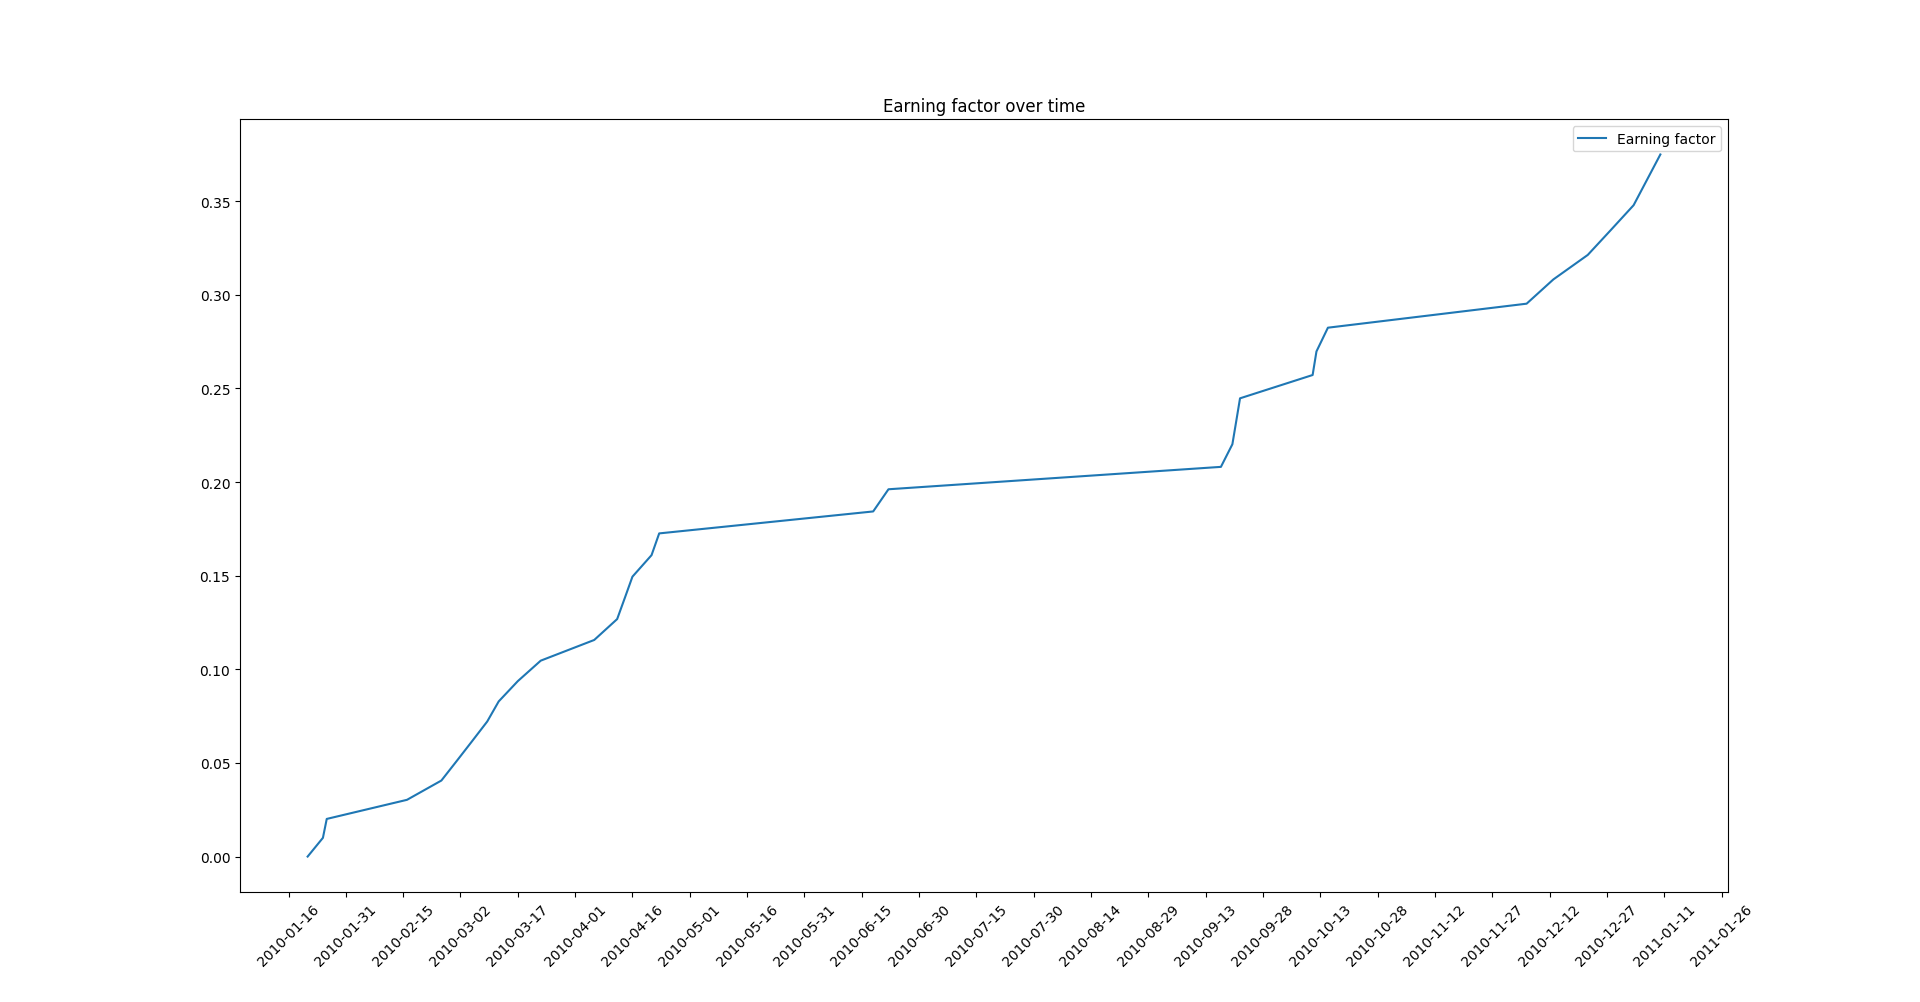
\includegraphics[width=\linewidth]{assets/simulations/single/sim_rn_aapl.png}
					\caption{RandomTradingAgent}
				}
				\end{figure}
				\begin{figure}[H]
				{
					\centering
					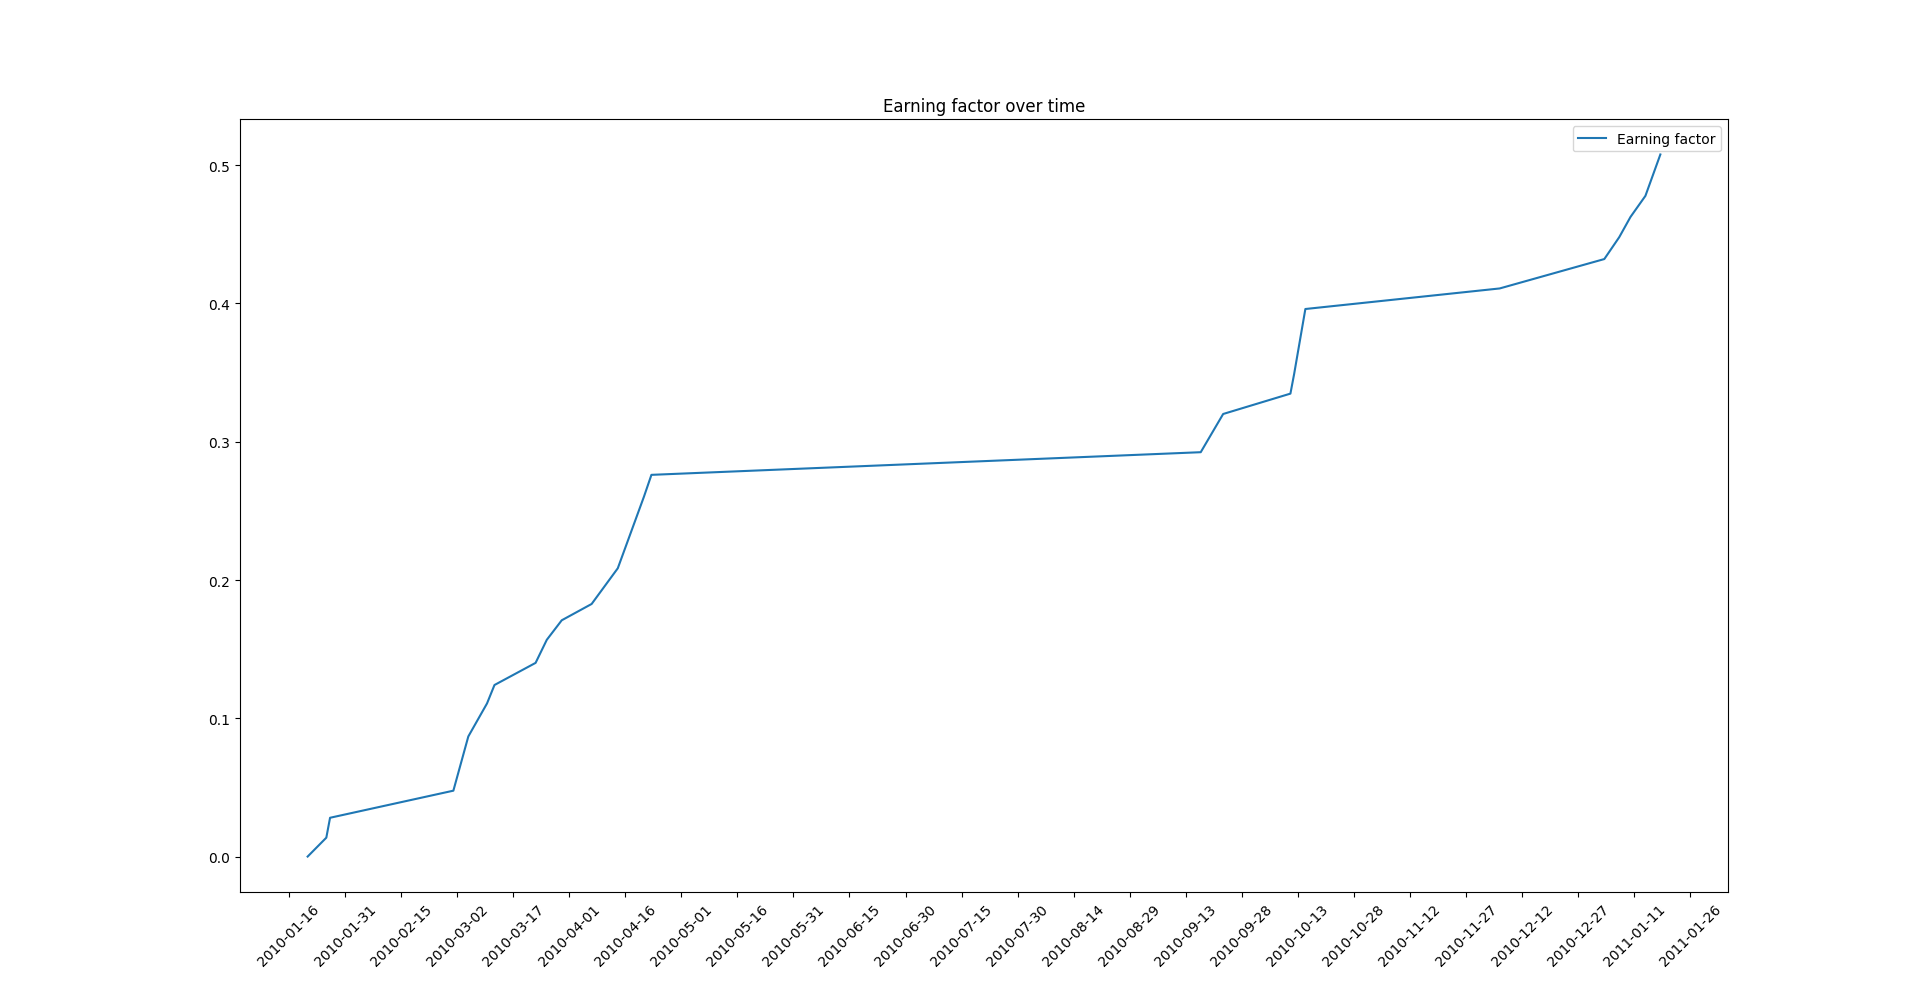
\includegraphics[width=\linewidth]{assets/simulations/single/sim_nh_aapl.png}
					\caption{TradingAgentSellAtHigh}
				}
				\end{figure}
				\begin{figure}[H]
				{
					\centering
					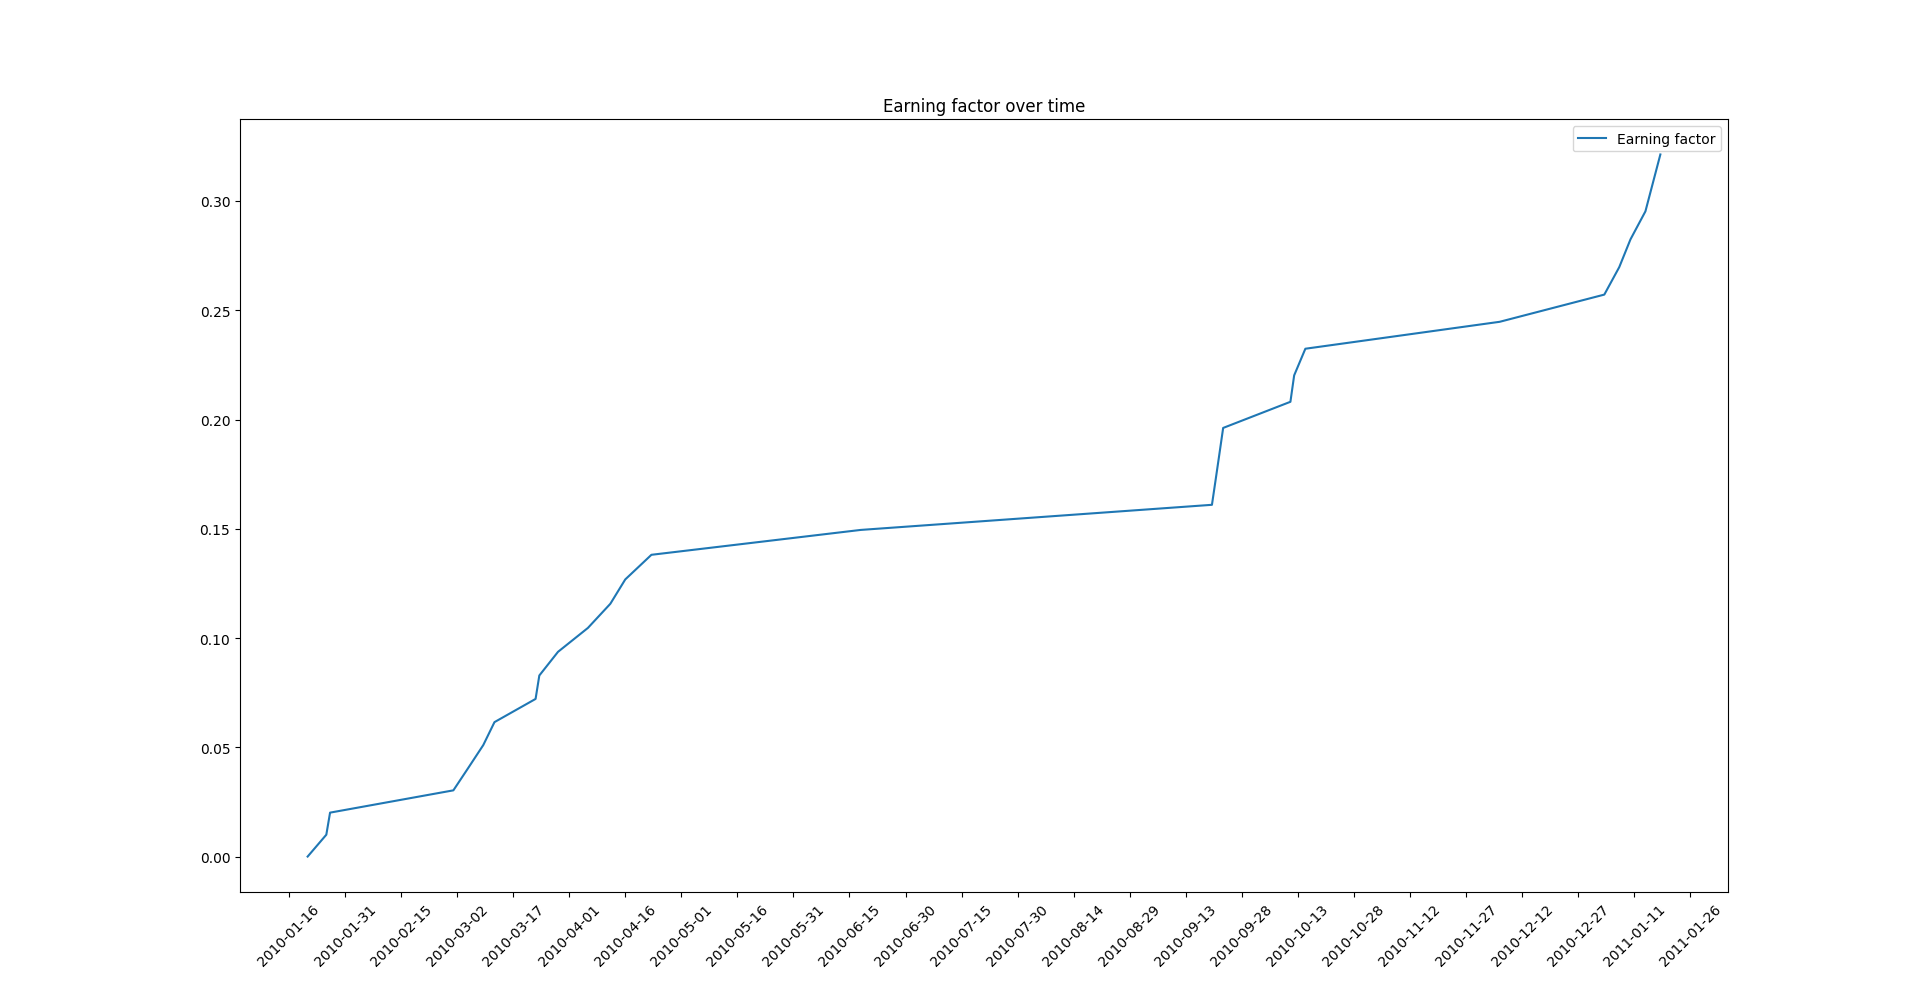
\includegraphics[width=\linewidth]{assets/simulations/single/sim_nt_aapl.png}
					\caption{TradingAgentSellAtTarget}
				}
				\end{figure}
				\begin{figure}[H]
				{
					\centering
					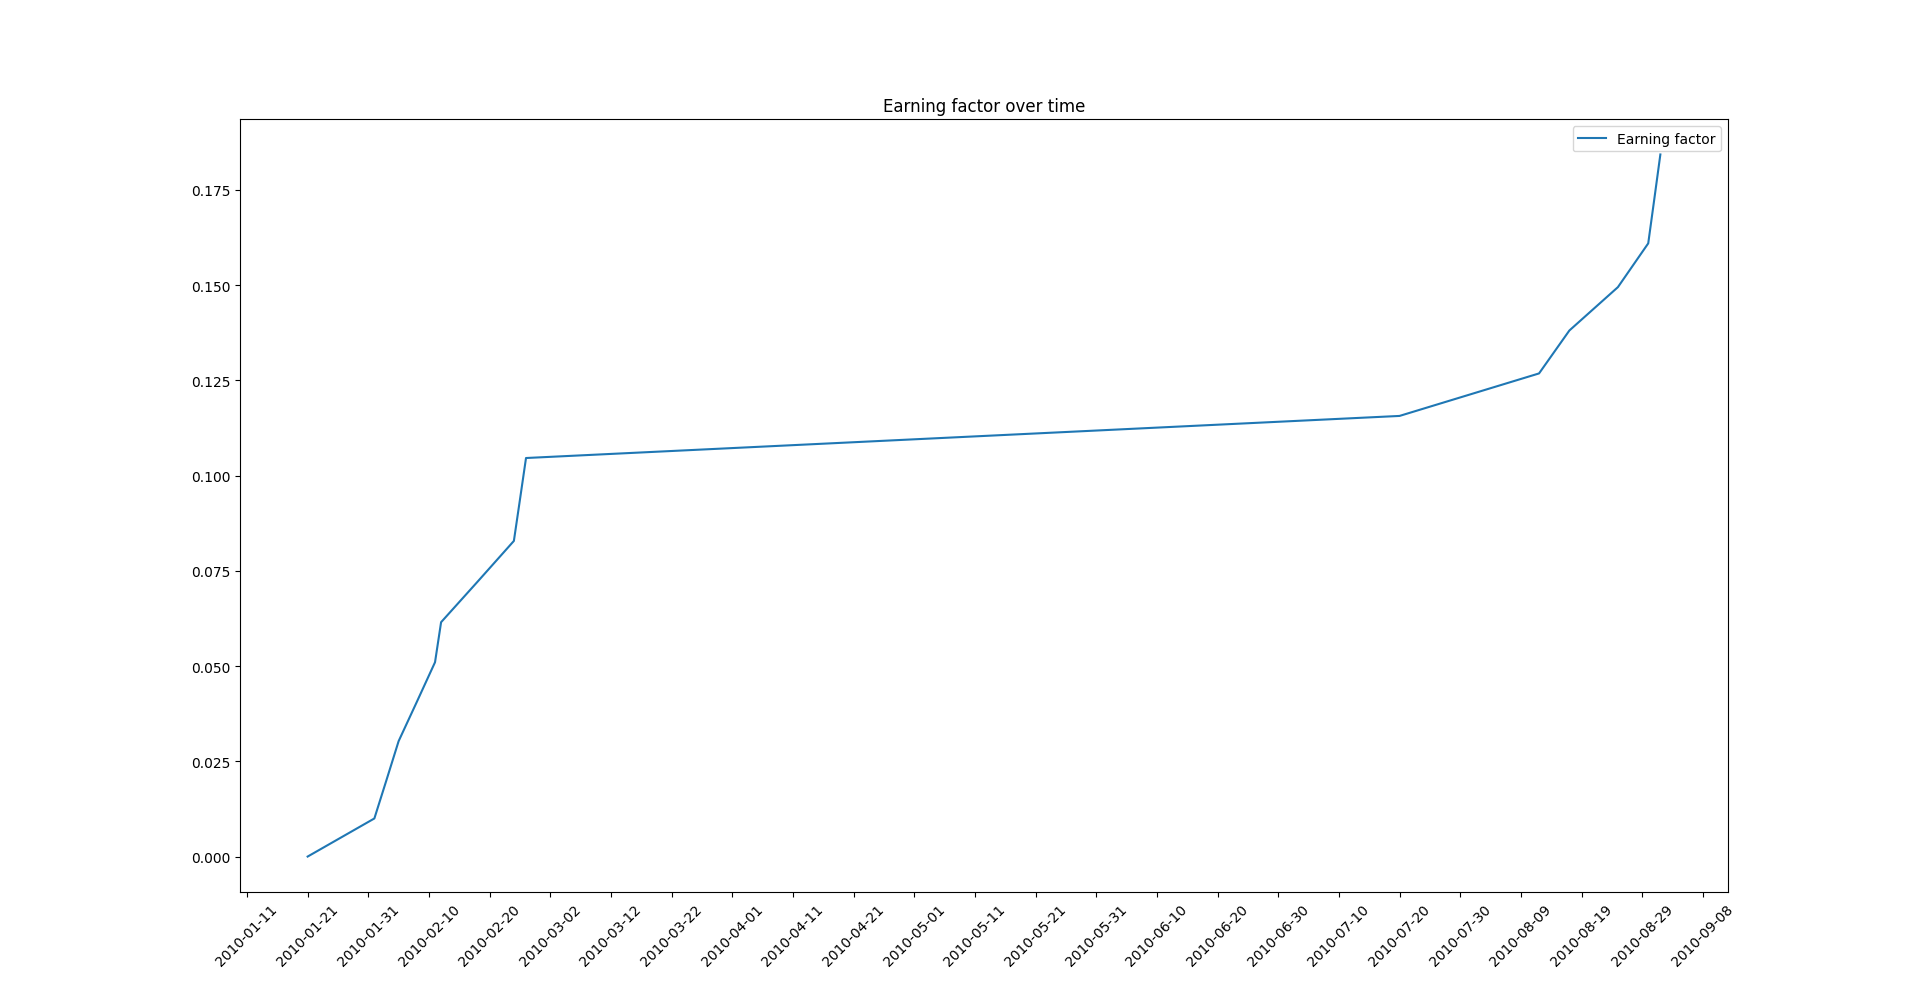
\includegraphics[width=\linewidth]{assets/simulations/single/sim_lr_aapl.png}
					\caption{LRTradingAgent}
				}
				\end{figure}
			\subsection{Agenti multi-titolo}
				\begin{figure}[H]
				{
					\centering
					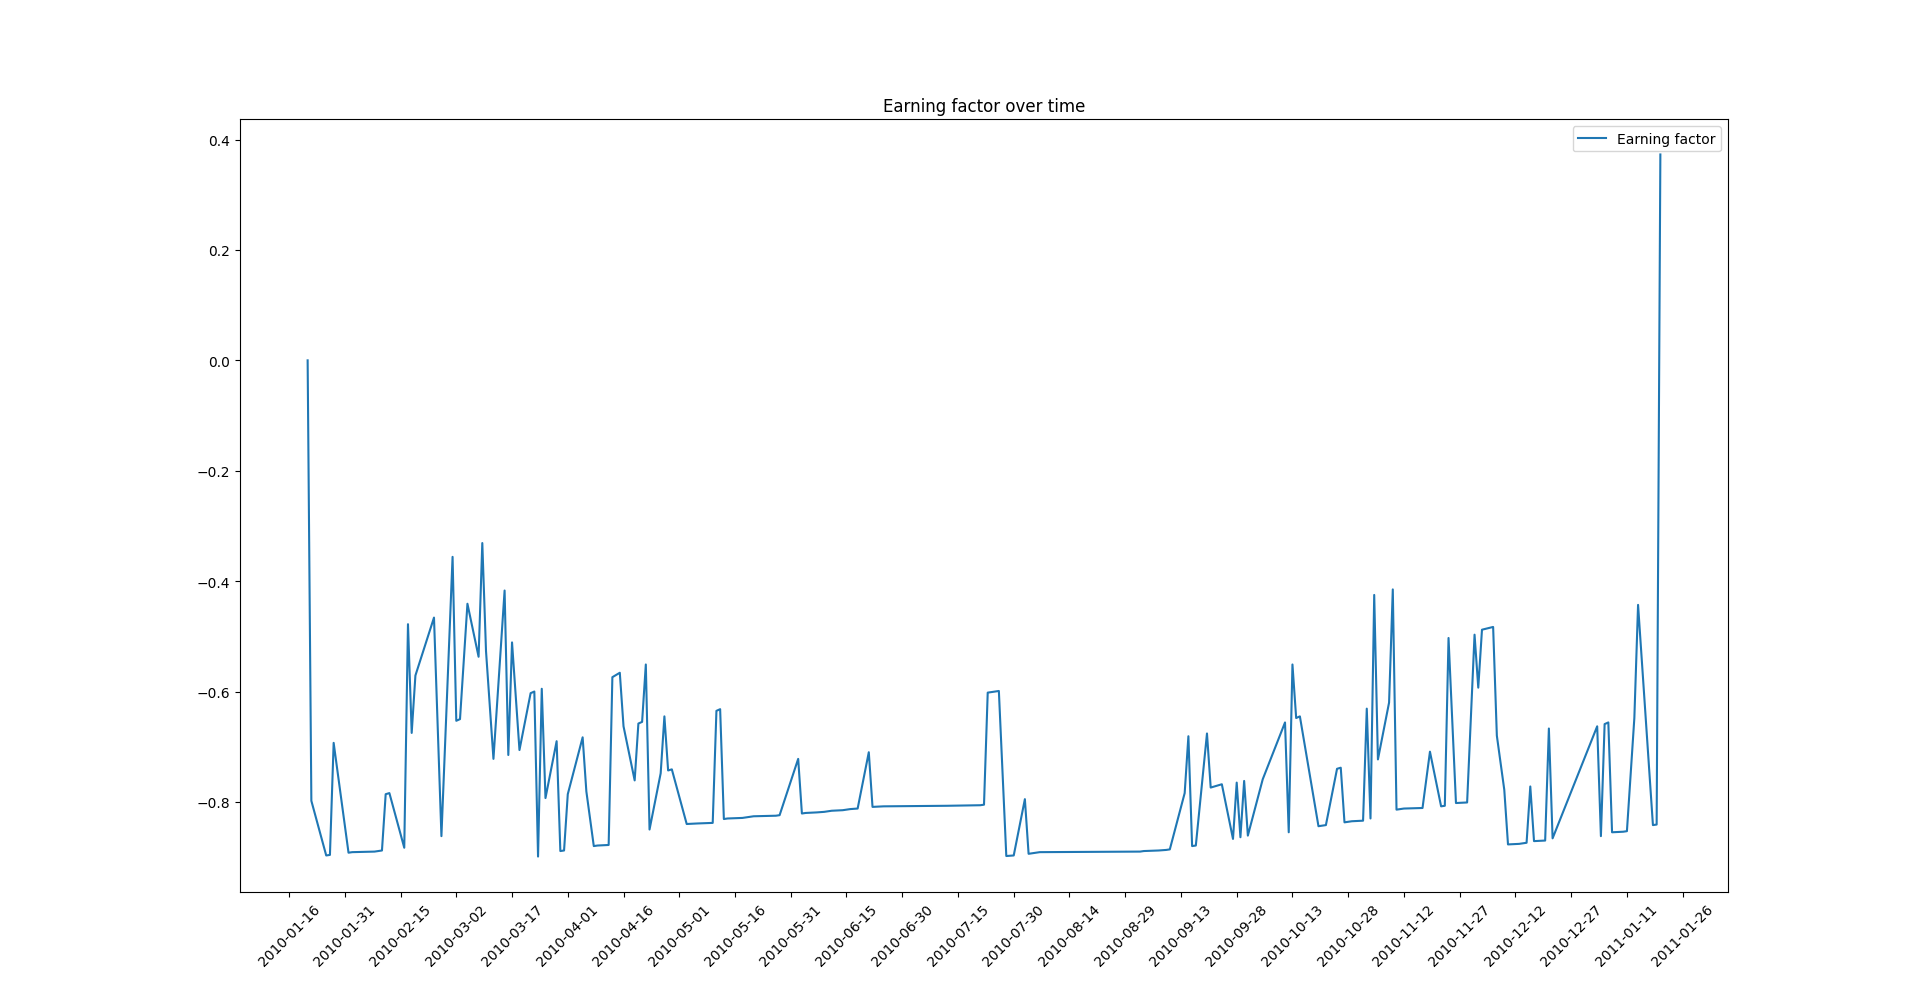
\includegraphics[width=\linewidth]{assets/simulations/multi/sim_rn_rn.png}
					\caption{RandomMultiAssetAgent}
				}
				\end{figure}
				\begin{figure}[H]
				{
					\centering
					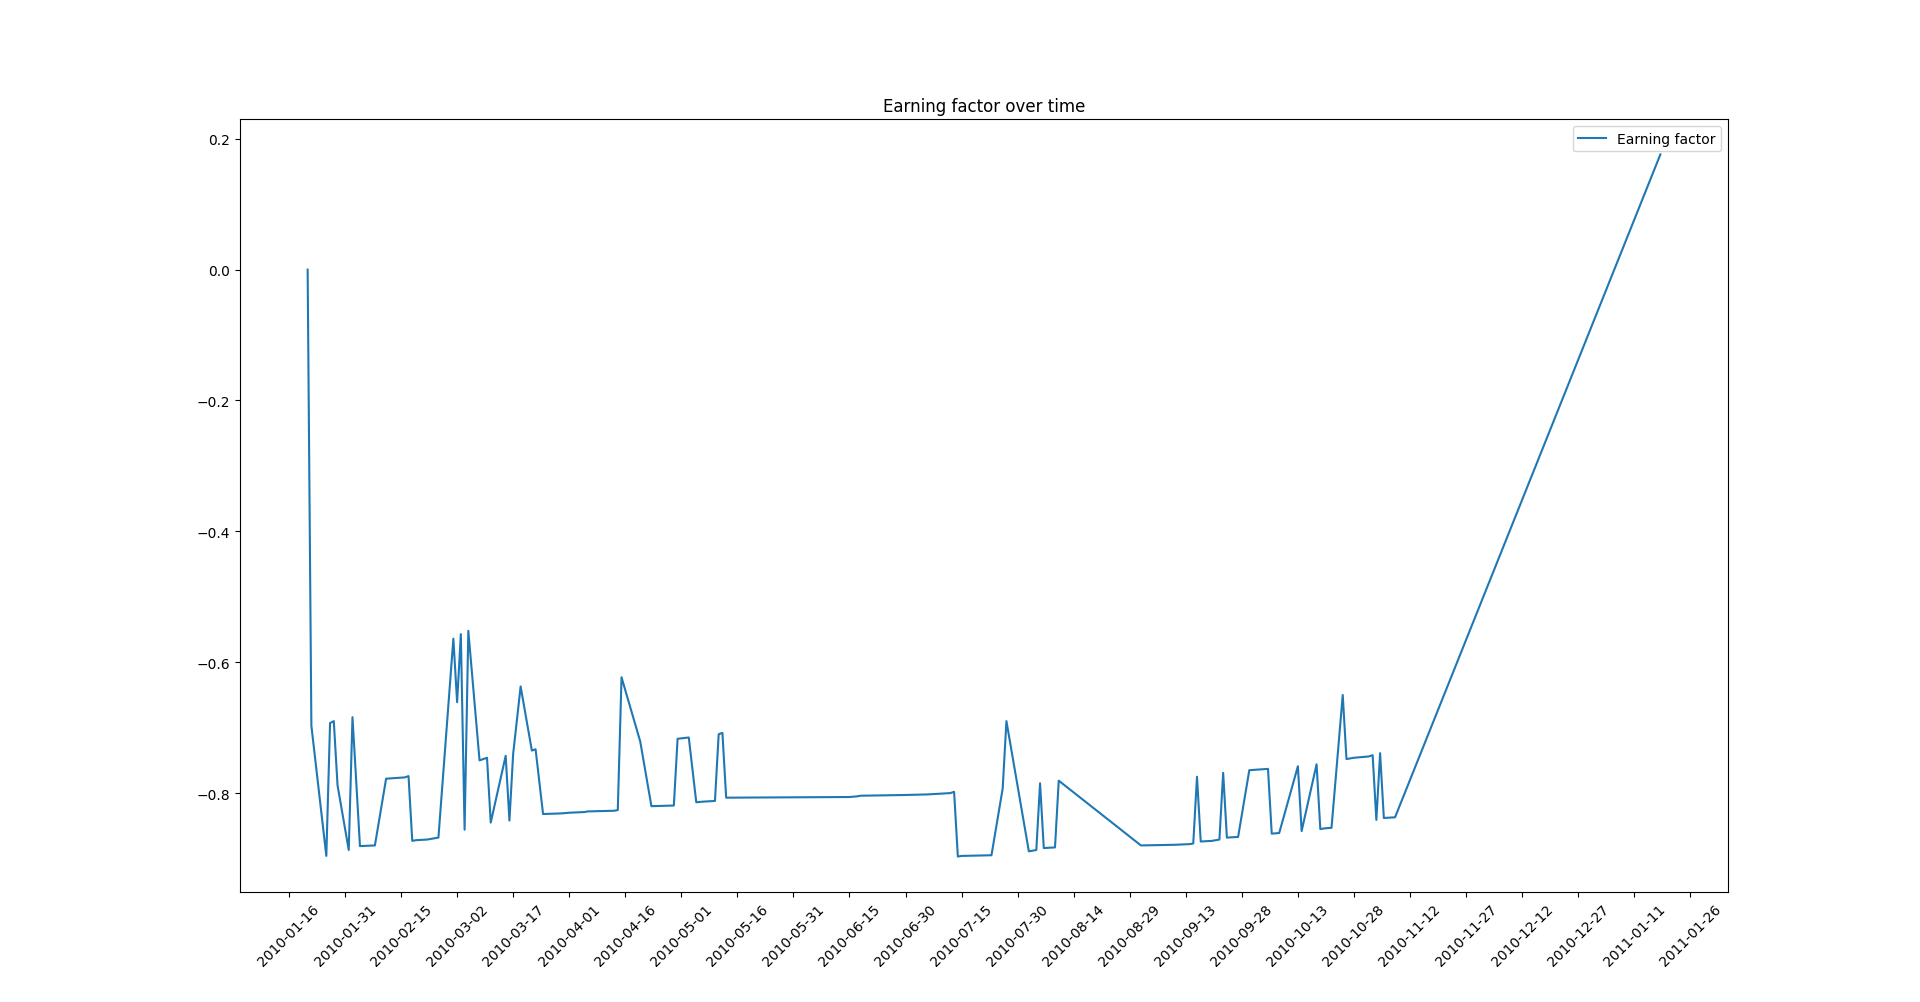
\includegraphics[width=\linewidth]{assets/simulations/multi/sim_rn_qo.png}
					\caption{QOptimMultiAssetAgent}
				}
				\end{figure}
				\begin{figure}[H]
				{
					\centering
					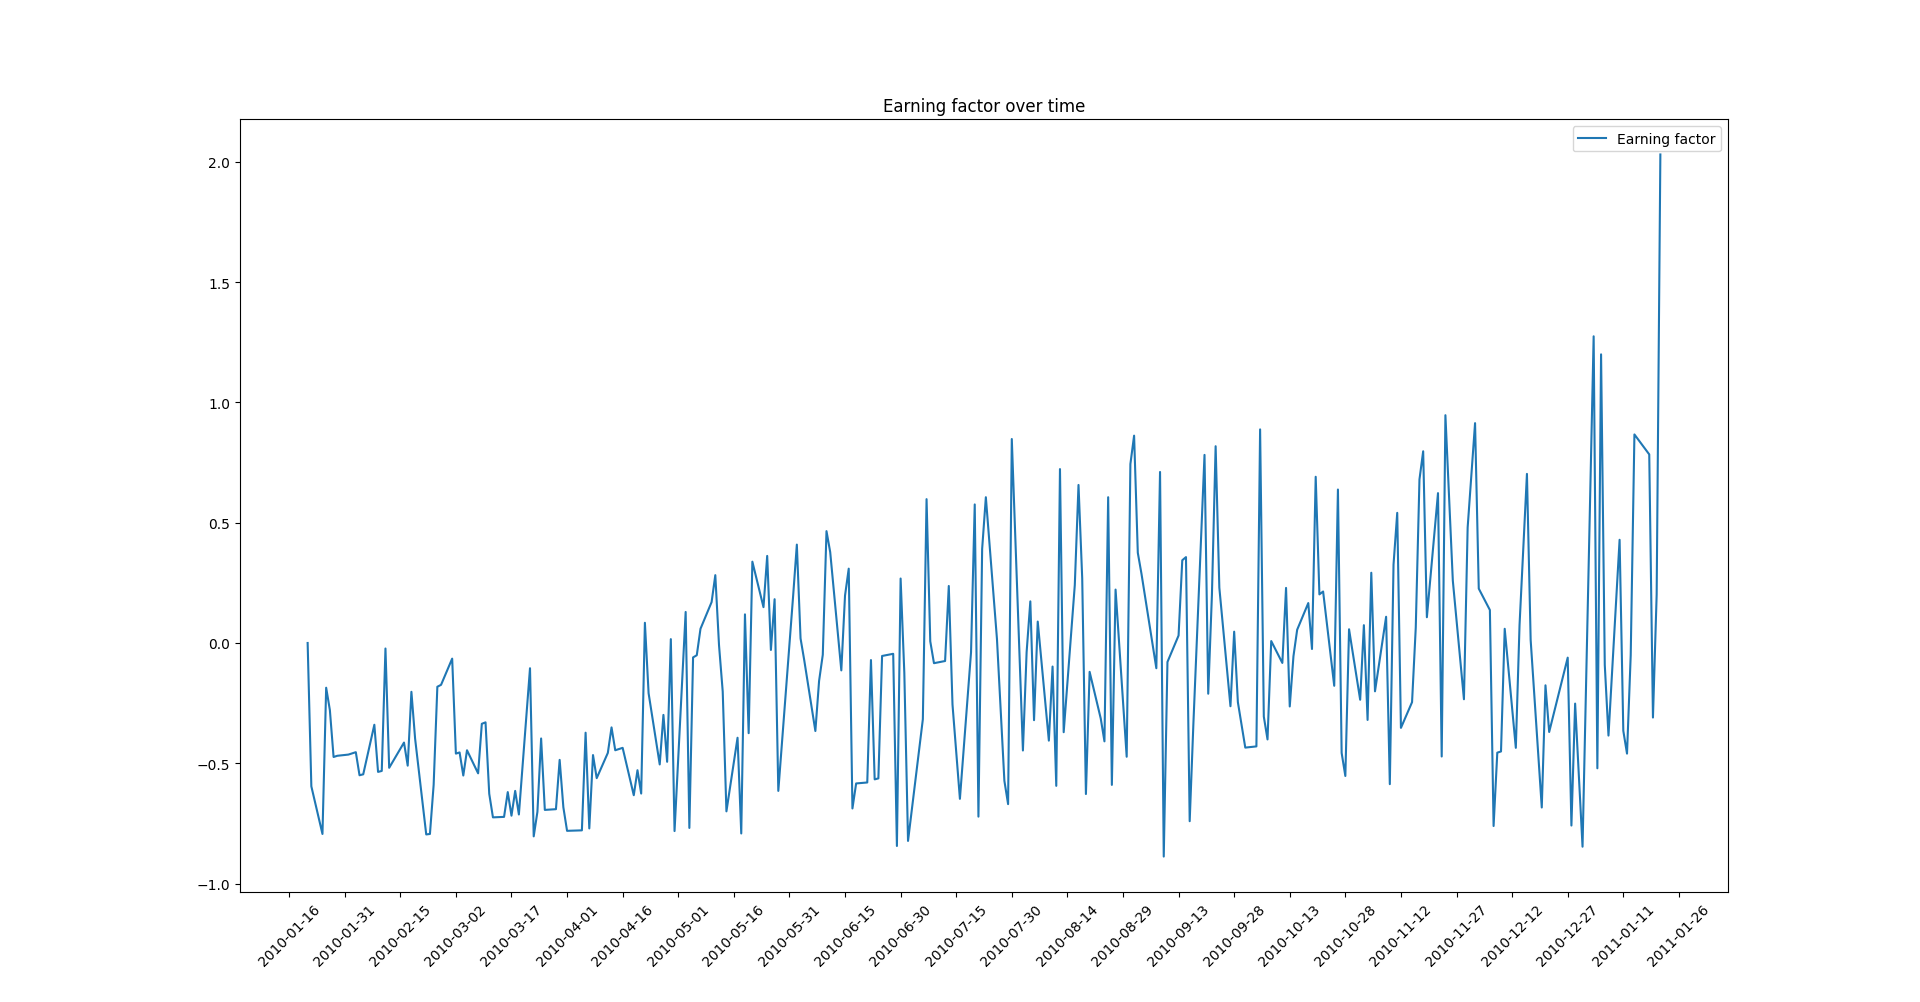
\includegraphics[width=\linewidth]{assets/simulations/multi/sim_lr_md.png}
					\caption{DeterministicMultiAssetAgent}
				}
				\end{figure}
				\begin{figure}[H]
				{
					\centering
					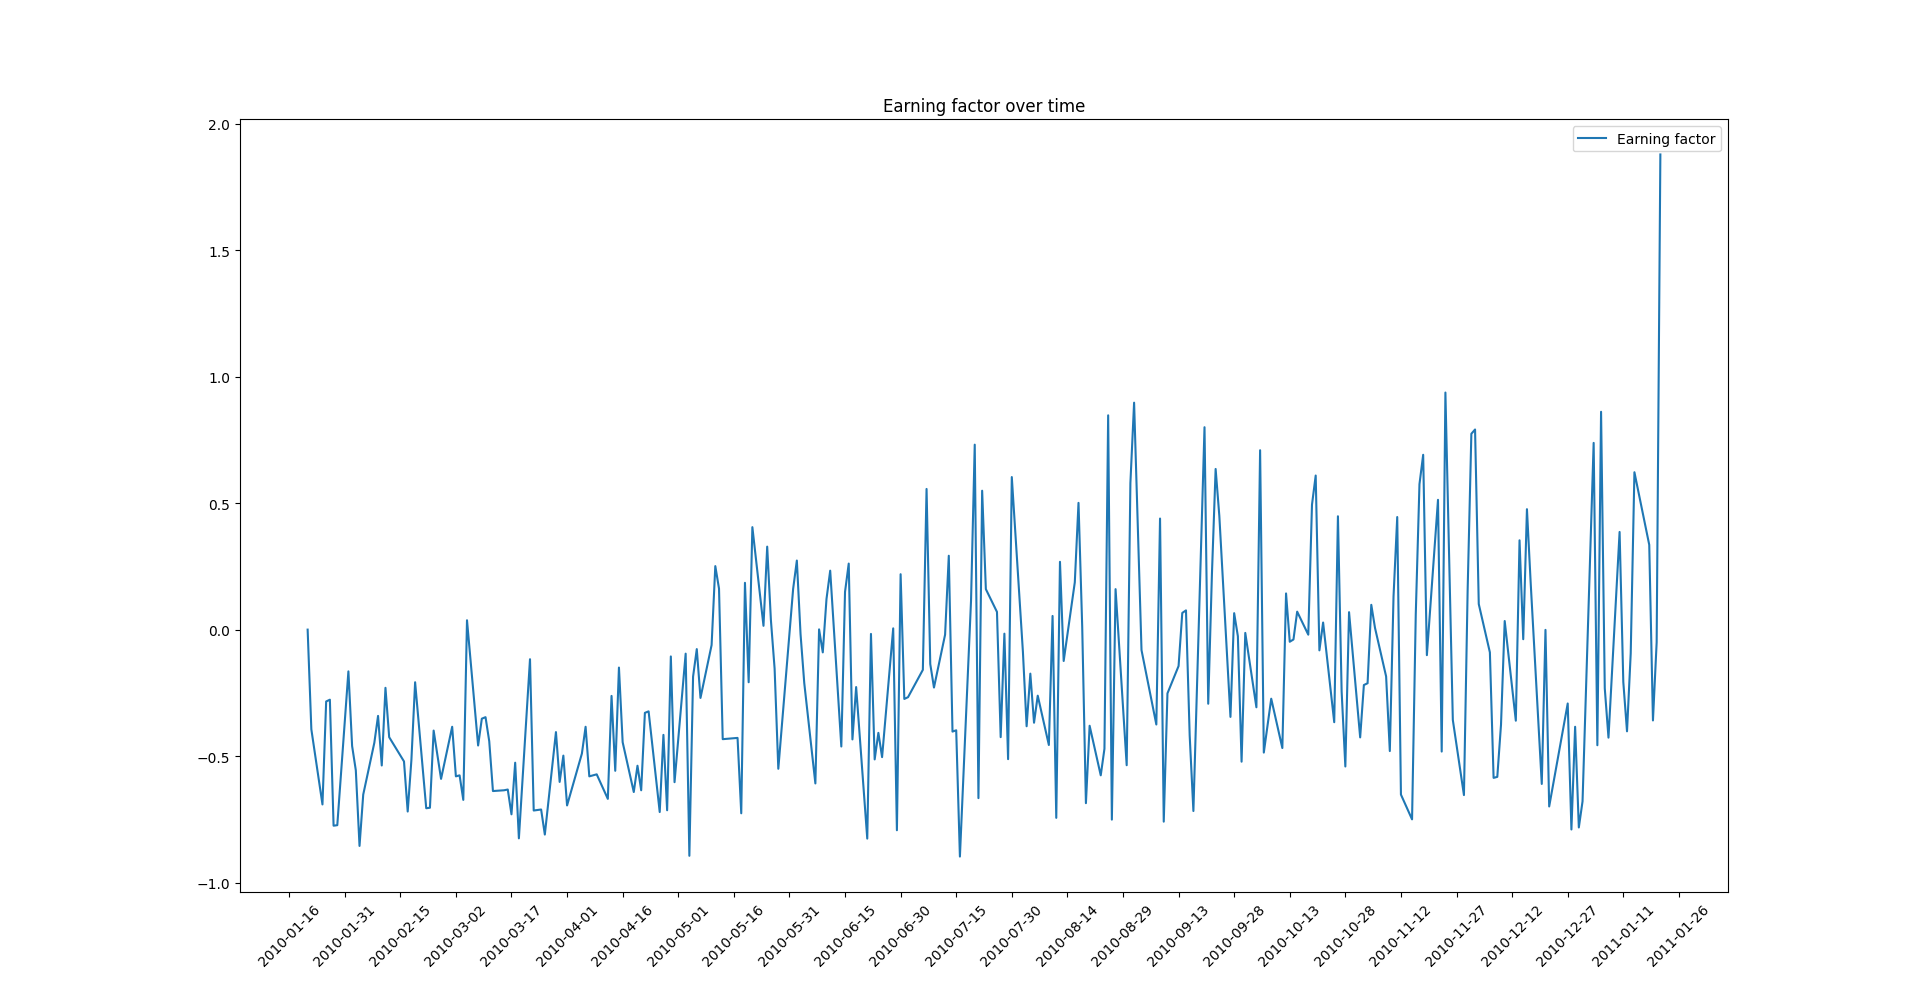
\includegraphics[width=\linewidth]{assets/simulations/multi/sim_lr_ms.png}
					\caption{StochasticMultiAssetAgent}
				}
				\end{figure}
		\section{Risultati}
			\subsection{Spiegazione delle variabili}
				\begin{itemize}
					\item $E^-$: Fattore di guadagno minimo alla fine dell'anno
					\item $E^+$: Fattore di guadagno massimo alla fine dell'anno
					\item $\mu(E)$: Fattore di guadagno medio alla fine dell'anno
					\item $\sigma(E)$: Deviazione standard del fattore di guadagno alla fine dell'anno
					\item $W^-$: Periodo di \textit{wait} minimo
					\item $W^+$: Periodo di \textit{wait} massimo
					\item $\mu(W)$: Periodo di \textit{wait} medio
					\item $\sigma(W)$: Deviazione standard del periodo di \textit{wait}
					\item $H^-$: Periodo di \textit{hold} minimo
					\item $H^+$: Periodo di \textit{hold} massimo
					\item $\mu(H)$: Periodo di \textit{hold} medio
					\item $\sigma(H)$: Deviazione standard del periodo di \textit{hold}
					\item $S^-$: Numero minimo di vendite in un anno
					\item $S^+$: Numero massimo di vendite in un anno
					\item $\mu(S)$: Numero medio di vendite in un anno
					\item $\sigma(S)$: Deviazione standard del numero di vendite in un anno
				\end{itemize}
			\subsection{Tabelle dei risultati}
				\label{sec:results}
				\input{progetto/results.tex}
		\section{Conclusioni}
			I risultati sono molto interessanti, sia perché confermano sperimentalmente ciò che è stato detto fino adesso, sia per le performance osservate. \\
			Bisogna però tenere a mente che le simulazioni e conseguentemente i risultati non tengono conto delle \textbf{\textit{transaction fees}} e le \textbf{\textit{overnight fees}}, che però possono essere
			stimate basandosi sul numero di vendite (e quindi di transazioni) e sui periodi di \textit{hold} (ad ogni giorno di \textit{hold} corrisponde ovviamente un \textit{overnight}). 
			\subsection{Agents mono-titolo}
				Il \textit{RandomTradingAgent}, implementato come \textit{proof of concept}, principalmente come metrica delle performance degli altri agent, si è mostrato invece sorprendentemente
				performante, con un guadagno medio essenzialmente in linea con gli altri agents, nonostante i bassi valori massimi. \\
				\textit{TradingAgentSellAtHigh} e \textit{TradingAgentSellAtTarget}, essenzialmente due facce della stessa medaglia, si sono comportati molto bene con $TP = 1\%$, degradando notevolmente
				le performance all'aumentare dello stesso. Ciò riflette il fatto che è relativamente raro che il prezzo aumenti di più dell'1\%, e la scarsa presenza di tali eventi nel dataset ha comportato
				che il modello non è in grado di prevedere in maniera affidabile tali eventi (per comprendere meglio ciò si rimanda alla \underline{\hyperref[fig:nn]{Figura 2.1}}). Per quanto riguarda la
				differenza tra i due approcci, le statistiche confermano quanto detto: la differenza di guadagno medio e la deviazione standard mostrano come vendere a \textit{high} abbia un maggiore potenziale
				di guadagno ma è decisamente meno robusto come approccio (soprattutto meno tollerante degli errori), ciò si nota anche nelle statistiche sul numero di vendite annuali e sul periodo di \textit{hold}
				(maggiore è l'errore, più cresce il periodo di \textit{hold} perché l'agent non può vendere). \\
				L'agent più interessante da discutere è \textit{LRTradingAgent}, nonostante il guadagno medio e la \textit{dry run} non promettano bene, dal numero di vendite ma soprattutto dal bassissimo periodo
				di \textit{hold} si nota come l'agent venda quasi sempre subito i titoli, che alla fine è il nostro scopo, e in ciò è il migliore in assoluto, confermandosi quindi anche come approccio più robusto
				su cui basare gli agents multi-titolo.
			\subsection{Agents multi-titolo}
				Per \textit{RandomMultiAssetAgent} vale quanto già detto per \textit{RandomTradingAgent}, è principalmente un agent di confronto il cui scopo è dimostrare la validità degli approcci discussi,
				cionostante si è comunque comportato discretamente, con un guadagno medio di circa il 30\%, ma la necessità di gestire più titoli ha mostrato la bassa robustezza di tale approccio, come evidente dal
				grafico. Lo stesso discorso vale per \textit{QOptimMultiAssetAgent}, che riesce a rendere quasi nulla la varianza del guadagno, ma questo aiuta poco in quanto il guadagno medio si attesta into al
				20\%, mentre le vendite medie sono, come ci si aspetta, inferiori all'agent "\textit{random}". \\
				Gli agents basati sulla regressione lineare invece, \textit{DeterministicMultiAssetAgent} e \textit{StochasticMultiAssetAgent}, dimostrano la vera potenza di questo approccio. Con il massimo fattore
				di guadagno fra tutti gli agent e, analogamente, il massimo numero di vendite annuali, si attestano come gli agent più efficienti. \\
				Per quanto riguarda le differenze tra i due, prevedibilmente \textit{DeterministicMultiAssetAgent} è quello con il maggiore guadagno ma anche la maggiore deviazione standard (escludendo il caso di
				$TP = 1\%$), a conferma di quanto detto in precedenza.
	\backmatter
	\cleardoublepage
	\phantomsection % Give this command only if hyperref is loaded
	\addcontentsline{toc}{chapter}{\bibname}
	\nocite{*}
	\bibliographystyle{plain}
	\bibliography{bibliography}
\end{document}
